\documentclass[a4paper,titlepage]{report}
\usepackage[T1]{fontenc}
\usepackage[utf8]{inputenc}
\usepackage[francais]{babel}
\usepackage{lmodern} % police véctorielle
\usepackage{pdfpages}
\usepackage{graphicx}
\usepackage{subfig}
\usepackage[hidelinks]{hyperref}
%\usepackage{url}
%\usepackage{array}
\usepackage{listings}
\usepackage{color}
% definition des marges
\usepackage[top=2.5cm,bottom=2.5cm,right=2.5cm,left=3.5cm]{geometry}
\usepackage{listingsutf8}
\usepackage{lscape}
\pagestyle{headings}

%retrait du numero des chapitre dans les sections
\makeatletter
\renewcommand{\thesection}{\@arabic\c@section}
\makeatother

\title{Rapport du projet de conception formelle :
	\begin{center}
		\textsc{Rodin 2014}
	\end{center}
}
\author{Jordan Aupetit, Salmane Bah, Timothée Sollaud \& Bruno Thiaolayel\\
	\\
	\\ \textsc{Université de Bordeaux}
}
\begin{document}
	\maketitle
	%\newpage
	\tableofcontents
	\newpage
	\thispagestyle{empty}	
	\newpage
	\pagenumbering{arabic} % Arabic page numbers from now on
% === Contenu =======================================================
\markboth{}{}
\section{Introduction}
	Dans le cadre de l'unité d'enseignement Conception Formelle du Master Informatique Génie Logiciel de l'université de Bordeaux, il nous a été proposé de formaliser le fonctionnement d'un bus arrivant à un arrêt.



\section{ContextUsagers}
	Nous avons défini un contexte \textbf{Usagers}, afin de représenter l'ensemble fini des usagers et la constante \textbf{BusCapacity}, représentant la capacité du bus.\\

\section{MachineBus0}
	La \textbf{MachineBus0} représente notre machine de base. Celle-ci assure la cohérence de l'enchaînement des événements et le respect de la règle de civisme proposée par le sujet. Ainsi, les usagers montent dans le bus qu'après que tous les passagers désirant descendre l'aient fait.\\
	
	\subsection{Les ensembles}
		\begin{description}
			\item[usagers\_a\_l\_arret] est un sous-ensemble des usagers représentant les usagers attendant au prochain arrêt.\\
			\item[passagers] est un sous-ensemble des usagers représentant les passagers du bus. Le cardinal de passager ne peut donc pas dépasser la capacité du bus.\\
			\item[passagers\_descendre] est un sous-ensemble des passagers représentant les passagers souhaitant descendre du bus au prochain arrêt.\\
		\end{description}
		
	\subsection{Les événements}
		Pour définir les gardes de nos événements, nous avons utilisé le booléen \textbf{bus\_roule}, qui est à vrai si le bus est en mouvement et à faux si le bus est à un arrêt.\\
		
		\begin{description}
			\item[bus\_arrive] est l'événement qui représente le fait que le bus se stoppe à un arrêt.
			
			Cet événement peut se produire uniquement si le bus roule. 
			%De plus, afin de ne pas s’arrêter pour rien, on s’assure que des usagers souhaitent monter ou que des passagers veulent descendre et enfin, qu’il y a de la place dans le bus. Ainsi lorsque des usagers attendent le bus à un arrêt, si celui-ci est plein et qu’aucun passager ne souhaite descende, il ne s’arrêtera pas.
			
			L'effet de l'événement est simplement d'arrêter le bus.\\
		
			\item[bus\_repart] est l'événement qui représente le fait que le bus repart d'un arrêt.
			
			Cet évènement peut se produire uniquement si le bus est arrêté. De plus, le bus ne doit repartir qu'une fois que tous les passagers souhaitant descendre l'ont fait et que les usagers attendant à l'arrêt soient tous montés ou que le bus soit plein. \\
			
			Dans notre première implémentation, nous avions fait en sorte que le bus puisse s'arrêter puis repartir puis s'arrêter à nouveau dans une boucle infinie. Cela permettait au bus de pouvoir parcourir une multitude d'arrêts, en faisant monter et descendre un certain nombre de passager à chaque fois.\\
			
			Dans notre seconde implémentation, afin de ne pas avoir une exécution infinie et ajouter un variant, nous avons décidé que le bus ne pourrait que s'arrêter et repartir une seule fois. De ce fait, l'évènement \textbf{bus\_repart} qui précisait que le bus roule à nouveau, indique maintenant que la simulation se termine. Donc, lorsqu'elle est terminée, il n'est plus possible de faire aucun évènement. Nous obtenons donc une deadlock afin d'obtenir une terminaison.
			


			\item[passager\_desc] est l'événement qui représente le fait qu'un passager descende du bus.
			
			Cet événement peut se produire uniquement si le bus est arrêté et qu'il y a au moins un passager qui souhaite descendre.
			
			L'effet de l'événement est de repasser le passager descendu en simple usager. \\
			
			\item[usager\_monte] est l'événement qui représente le fait qu'un passager monte dans le bus.
			
			Cet événement ne peut se produire que si le bus est arrêté, qu'au moins un usager souhaite monter et que tous les passagers voulant descendre l'ont fait.
			
			L'effet de cet événement est de déplacer l'usager de l'ensemble des usagers attendant à l'arrêt vers l'ensemble représentant les passagers du bus.\\
		
			\item[usager\_arrive] est l'événement représentant un usager arrivant à un arrêt, dans l'espoir de prendre le prochain bus.
			
			Cet événement peut se produire à tout moment, tant qu'il reste au moins un usager qui n'est ni à un arrêt, ni déjà passager du bus.
			
			L'effet de l'événement est simplement d'ajouter l'usager à la liste des usagers souhaitant monter.\\
			
			\item[passager\_veut\_desc] est l'évènement qui représente le fait qu'un passager du bus veuille descendre au prochain arrêt.
			
			Cet évènement peut se produire uniquement si le bus roule et qu'il reste des passagers n'ayant pas déjà décidé de descendre.
			
			L'effet de l'évènement est d'ajouter le passager à l'ensemble des passagers souhaitant descendre.\\
		\end{description}

	\subsection{Le variant}
		Maintenant que notre machine se termine nous avons réussi à mettre en place un variant. Pour ce faire, nous avons rajouté un contexte qui permet de convertir un booléen en entier qui va nous servir dans notre variable. Ce contexte s'appelle \textbf{BoolToInt}. Nous avons choisis comme variant le nombre de passagers voulant descendre, auquel on ajoute un entier représentant l'état de la simulation (0 pour terminée, sinon 1). Nous avons rajouté cet entier afin que le variant ait la valeur nulle dès que la simulation est terminée. Dans le cas contraire, le variant aurait eu la valeur nulle avant de repartir de l'arrêt. Nous avons réussi à prouver ce variant, ce qui démontre que notre machine se termine quoi qu'il arrive.
	
\section{MachineBus1}
	La \textbf{MachineBus1} est le premier raffinement de la machine de base \textbf{MachineBus0}. Elle intègre la gestion d'usagers prioritaires.\\
		
	\subsection{Les ensembles}
		Dans cette machine, les ensembles décrits précédemment n'ont pas été modifiés, excepté \textbf{usagers\_à\_l\_arrêt}, qui se décompose à présent en deux ensembles afin de gérer des usagers prioritaires :
		 	
		\begin{description}
			\item[usagers\_a\_l\_arret\_prioritaire], qui représente la partition des usagers prioritaires attendant au prochain arrêt.
			\item[usagers\_a\_l\_arret\_non\_prioritaire], qui représente la partition des usagers non prioritaires attendant au prochain arrêt.\\
		\end{description}
				
	\subsection{Les évènements}
		On retrouve dans ce raffinement la plupart des évènements de la machine d'origine, dans lesquels l'ensemble \textbf{usagers\_a\_l\_arret} a été remplacé par l'union des ensembles \textbf{usagers\_a\_l\_arret\_prioritaire} et \textbf{usagers\_a\_l\_arret\_non\_prioritaire}.\\
		
		L'évènement \textbf{usager\_arrive} a été décomposé en deux évènements, afin de gérer les priorités :
		\begin{description}
			\item[usagers\_arrive\_prioritaire] est l'évènement représentant un usager prioritaire arrivant à un arrêt, dans l'espoir de prendre le prochain bus.
			
			Cet évènement peut se produire à tout moment, tant qu'il reste au moins un usager qui n'est ni en attente à un arrêt, ni déjà passager du bus.
			
			L'effet de l'évènement est simplement d'ajouter l'usager à la liste des usagers prioritaires souhaitant monter.
			
			\item[usagers\_arrive\_non\_prioritaire] est l'évènement représentant un usager non prioritaire arrivant à un arrêt, dans l'espoir de prendre le prochain bus.
			
			Cet évènement peut se produire à tout moment, tant qu'il reste au moins un usager qui n'est ni en attente à un arrêt, ni déjà passager du bus.
			
			L'effet de l'évènement est simplement d'ajouter l'usager à la liste des usagers non prioritaires souhaitant monter.\\
		\end{description}
		

		De même, afin de gérer les priorités, l'évènement \textbf{usager\_monte} a été décomposé en deux évènements:
		
		\begin{description}
			\item[usagers\_monte\_prioritaire] est l'évènement qui représente le fait qu'un passager prioritaire monte dans le bus.
			
			Cet évènement ne peut se produire que si le bus est arrêté, qu'au moins un usager prioritaire souhaite monter et que tous les passagers voulant descendre l'ont fait.
			
			L'effet de cet évènement est de déplacer l'usager prioritaire attendant à l'arrêt vers l'ensemble des passagers du bus.\\
			
			\item[usagers\_monte\_non\_prioritaire] est l'évènement qui représente le fait qu'un passager non prioritaire monte dans le bus.
			
			Cet évènement ne peut se produire que si le bus est arrêté, qu'au moins un usager non prioritaire souhaite monter, que tous les passagers voulant descendre l'ont fait et que tous les passagers prioritaires sont montés.
			
			L'effet de cet évènement est de déplacer l'usager non prioritaire attendant à l'arrêt vers l'ensemble des passagers du bus.\\
		\end{description}
		
		Nous avons rajouté un dernier évènement permettant à notre simulation de ne pas se terminer. Celui-ci s'appelle \textbf{idle}. Il est appelé en boucle à partir du moment où la simulation se termine ou plus précisément, après l'évènement \textbf{bus\_repart}. Cela nous permet d'ignorer les deadlocks hors simulation. 
		
		

\subsection{DeadLock Freeness}
	Afin de prouver que notre premier raffinement n'a pas de situations	de blocages, nous avons vérifié que le modèle n'a pas de deadlocks évidentes à l'aide du plug-in "ProB". Vous pouvez voir nos résultats sur l'image ci-dessous. Afin de garantir ce résultat, nous avons rajouté un théorème ou DeadLock Freeness. Nous avons réussi à le prouver, ce qui justifie que cette machine n'a aucun blocage. \\
	
	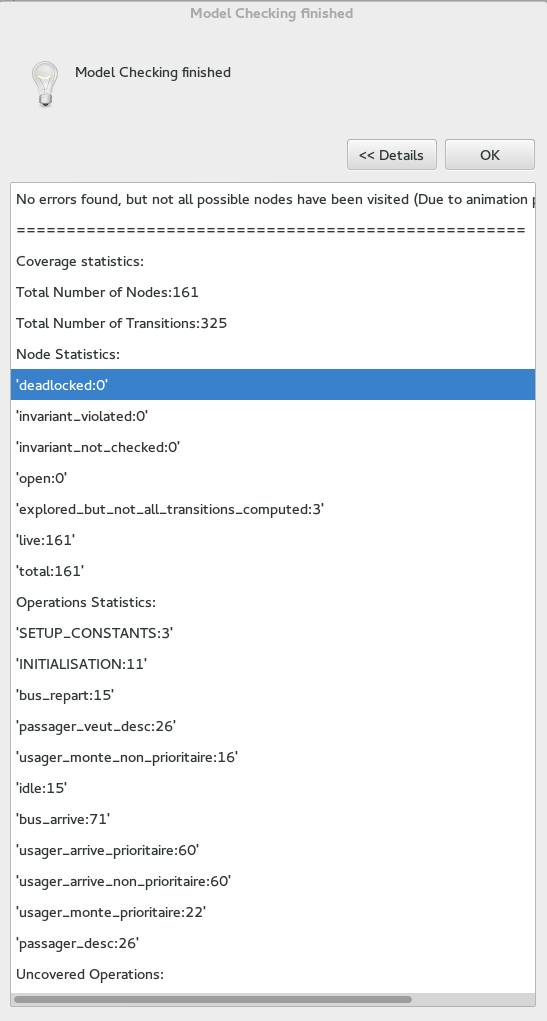
\includegraphics[width=\textwidth]{checkMachineBus1.png}
	
	
\section{MachineBus2}	
	La \textbf{MachineBus2} est le second raffinement de la machine de base \textbf{MachineBus0}. Elle intègre la notion de file sur les usagers non prioritaires.\\
	
	
	
		
\end{document}
